% !TEX program = xelatex
\documentclass[a4paper,11.5pt,UTF8]{ctexart}
\usepackage{a4}
\usepackage{amsmath, amssymb, amsthm, graphicx, xspace,array,url}
\usepackage{setspace}
\usepackage{float}
\usepackage{listings,color,xcolor,fontspec}

\CTEXsetup[format={\Large\bfseries}]{section}

\lstset{
	columns=fixed,       
	numbers=left,                                        % 在左侧显示行号
	numberstyle=\tiny\color{gray},                       % 设定行号格式
	frame=none,                                          % 不显示背景边框
	backgroundcolor=\color[RGB]{245,245,244},            % 设定背景颜色
	keywordstyle=\color[RGB]{40,40,255},                 % 设定关键字颜色
	numberstyle=\footnotesize\color{darkgray},           
	commentstyle=\it\color[RGB]{0,96,96},                % 设置代码注释的格式
	stringstyle=\rmfamily\slshape\color[RGB]{128,0,0},   % 设置字符串格式
	showstringspaces=false,                              % 不显示字符串中的空格
	language=c++,                                        % 设置语言
}

\title{Project 1}
\author{张卓涵 3190101161}
\usepackage[a4paper,left=20mm,right=20mm,top=30mm,bottom=20mm]{geometry}

\newtheorem{example}{\hspace{2em}例}{}
\newtheorem{remark}{\hspace{2em}注}{}
\newtheorem{thm}{\hspace{2em}定理}{}
\newtheorem{lemma}{\hspace{2em}引理}{}

\begin{document}
\begin{figure}[t]
\begin{minipage}[h]{0.25\linewidth}
	
\includegraphics[width=4.0cm]{./picture/ZJU2.jpeg}
\end{minipage}
\hfill
\begin{minipage}[h]{.7\linewidth}
	\begin{flushright}
			\Large{微分方程数值解
				\vspace{3mm}	\\
				   2022 春
				\vspace{3mm}	\\
				   张卓涵 \hspace{3mm}3190101161}
	\end{flushright}
\end{minipage}
\rule{\linewidth}{0.1em}
\end{figure}
\begin{center}
	\huge{\textbf{Project 1}}
\end{center}
\begin{large}
	
\section{Boundary Conditions in the Json files}
\par 一共有三个json文件,分别测试了Dirichlet,Neumann和Mixed边值条件下的计算结果与误差。
	
\section{Errors and Convergence Rates}
\subsection{The first function}
\par 测试的第一个函数是
$$u(x,y) = e^{y+\sin(x)}$$
测试中不规则定义域中的圆选取为$(x-\frac{2}{3})^2+(y-\frac{1}{2})^2=\frac{1}{16}$.
\par 对第一种边值条件,
\begin{center}
\begin{tabular}{|c|c|c|c|c|c|c|}
	\hline
	& \multicolumn{3}{c|}{regular domin} & \multicolumn{3}{c|}{irregular domin} \\
	\hline
	n & 1-norm & 2-norm & $\infty$-norm & 1-norm &	2-norm& $\infty$-norm \\
	\hline
	8& 0.00203806 & 0.000979757 & 0.000713907 & 0.000515528 & 0.000321185 & 0.000484398 \\
	\hline
	16& 0.000986439 & 0.000314313 & 0.000156243 & 0.000231921 &8.57369e-05	&7.30423e-05\\
	\hline
	32& 0.000481015 & 0.000105927 & 3.675e-05 & 0.000114244 &2.94551e-05&1.32204e-05\\
	\hline
	64& 0.000237115 & 3.65733e-05 & 8.89928e-06 & 5.78276e-05 &1.0584e-05	&3.39176e-06 \\
	\hline
\end{tabular}
\end{center}
可以看到,对于Dirchlet条件来说,因为采用了2阶准确的推导方式,$\infty$-norm基本是呈2阶速度收敛的.
\par 对第二种边值条件,
\begin{center}
\begin{tabular}{|c|c|c|c|c|c|c|}
	\hline
	& \multicolumn{3}{c|}{regular domin} & \multicolumn{3}{c|}{irregular domin} \\
	\hline
	n & 1-norm & 2-norm & $\infty$-norm & 1-norm &	2-norm& $\infty$-norm \\
	\hline
	8& 0.0287087 & 0.0127368 & 0.00954259 & 0.00984642 & 0.00507879 & 0.00471488 \\
	\hline
	16& 0.0112275 & 0.00361008 & 0.00207687 & 0.00372914 &0.00141041	&0.00107647\\
	\hline
	32& 0.00499464 & 0.00114854 & 0.000486224 & 0.00164286 &0.000442976&0.000256925\\
	\hline
	64& 0.00235809 & 0.000385649 & 0.000117726 & 0.000765231 &0.000146782&6.24026e-05 \\
	\hline
\end{tabular}
\end{center}
可以看到,对于Neumann条件来说(此时圆上仍然是Dirchlet条件),同样因为采用了2阶准确的推导方式,$\infty$-norm的收敛速度几乎也是2阶的.
\par 对第三种边值条件,
\begin{center}
\begin{tabular}{|c|c|c|c|c|c|c|}
	\hline
	& \multicolumn{3}{c|}{regular domin} & \multicolumn{3}{c|}{irregular domin} \\
	\hline
	n & 1-norm & 2-norm & $\infty$-norm & 1-norm &	2-norm& $\infty$-norm \\
	\hline
	8& 0.0534236 & 0.0235603 & 0.0170158 & 0.899454 & 0.35012 & 0.217818 \\
	\hline
	16& 0.0214377 & 0.00679174 & 0.00370531 & 0.516738 &0.153652	&0.0721617\\
	\hline
	32& 0.00965257 & 0.00217846 & 0.000867512 & 0.368703 &0.0810323&0.0318423\\
	\hline
	64& 0.00458538 & 0.000734409 & 0.000210047 & 0.334953 &0.0537717&0.0147153 \\
	\hline
\end{tabular}
\end{center}
这里,因为对圆上的法向导数的拟合采用的是1阶准确表达式,所以$\infty$-norm的收敛速度变为了近似1阶.
\par 绘制出在第二个边值条件及不规则定义域下,$n=64$时拟合出的函数图像如下:
\begin{figure}[htbp]
	\centering
	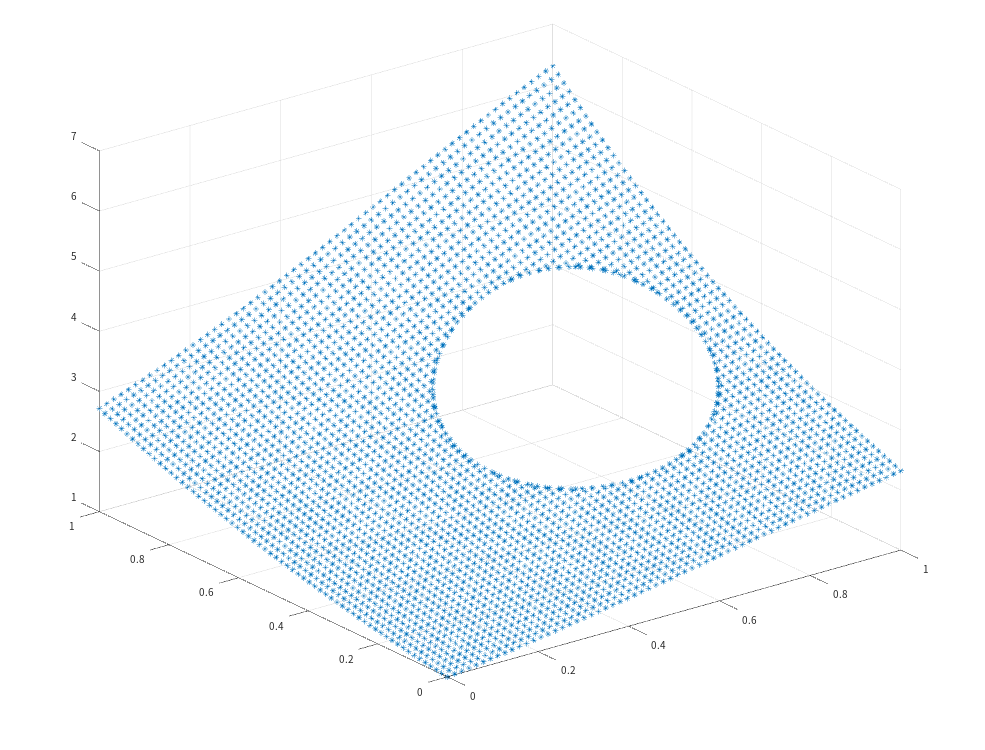
\includegraphics[width=0.8\textwidth,height=0.6\textwidth]{../output/image/image1.png}
\end{figure}

\subsection{The second function}
\par 测试的第二个函数是
$$ u(x,y)=\sin(x)+\sin(y) $$
测试中不规则定义域中的圆选取为$(x-1)^2+(y-\frac{1}{2})^2=(\frac{3}{4})^2$.
\par 对第一个边值条件,
\begin{center}
\begin{tabular}{|c|c|c|c|c|c|c|}
	\hline
	& \multicolumn{3}{c|}{regular domin} & \multicolumn{3}{c|}{irregular domin} \\
	\hline
	n & 1-norm & 2-norm & $\infty$-norm & 1-norm &	2-norm& $\infty$-norm \\
	\hline
	8& 0.000366633 & 0.000172369 & 0.000119539 & 7.03303e-05 & 7.02674e-05 & 9.89743e-05 \\
	\hline
	16& 0.000179819 & 5.56823e-05 & 2.61814e-05 & 2.28184e-05 &1.31254e-05	&1.22428e-05\\
	\hline
	32& 8.79452e-05 & 1.87928e-05 & 6.17646e-06 & 6.9716e-06 &2.63643e-06&1.61219e-06\\
	\hline
	64& 4.33824e-05 & 6.49075e-06 & 1.49821e-06 & 2.37587e-06 &6.14344e-07&2.3733e-07 \\
	\hline
\end{tabular}
\end{center}
\par 对第二个边值条件,
\begin{center}
\begin{tabular}{|c|c|c|c|c|c|c|}
	\hline
	& \multicolumn{3}{c|}{regular domin} & \multicolumn{3}{c|}{irregular domin} \\
	\hline
	n & 1-norm & 2-norm & $\infty$-norm & 1-norm &	2-norm& $\infty$-norm \\
	\hline
	8& 0.00572595 & 0.00248577 & 0.00186976 & 0.000261611 & 0.000249722 & 0.000358033 \\
	\hline
	16& 0.00229841 & 0.000719216 & 0.000407668 & 0.000101533 &6.76248e-05	&9.38843e-05\\
	\hline
	32& 0.00103217 & 0.000230862 & 9.54724e-05 & 4.20421e-05 &2.05855e-05&2.32333e-05\\
	\hline
	64& 0.000489496 & 7.78433e-05 & 2.31178e-05 & 1.90082e-05 &6.71804e-06&5.74242e-06 \\
	\hline
\end{tabular}
\end{center}
\par 对第三个边值条件,
\begin{center}
\begin{tabular}{|c|c|c|c|c|c|c|}
	\hline
	& \multicolumn{3}{c|}{regular domin} & \multicolumn{3}{c|}{irregular domin} \\
	\hline
	n & 1-norm & 2-norm & $\infty$-norm & 1-norm &	2-norm& $\infty$-norm \\
	\hline
	8& 0.00585159 & 0.00253797 & 0.00190105 & 0.0227054 & 0.0128118 & 0.00977785 \\
	\hline
	16& 0.00235335 & 0.000735311 & 0.000414269 & 0.0131987 &0.0062158	&0.00588506\\
	\hline
	32& 0.00105914 & 0.000236334 & 9.70077e-05 & 0.0109632 &0.00394731&0.0030329\\
	\hline
	64& 0.000502869 & 7.97495e-05 & 2.3489e-05 & 0.00956432 &0.00253507&0.00155869 \\
	\hline
\end{tabular}
\end{center}
\par 对前两个边值条件,$\infty$-norm基本呈2阶收敛.对第三个边值条件,不规则定义域上的误差的$\infty$-norm呈1阶收敛速度.
\par 绘制出在第二个边值条件及不规则定义域下,$n=64$拟合出的函数图像如下:
\begin{figure}[H]
	\centering
	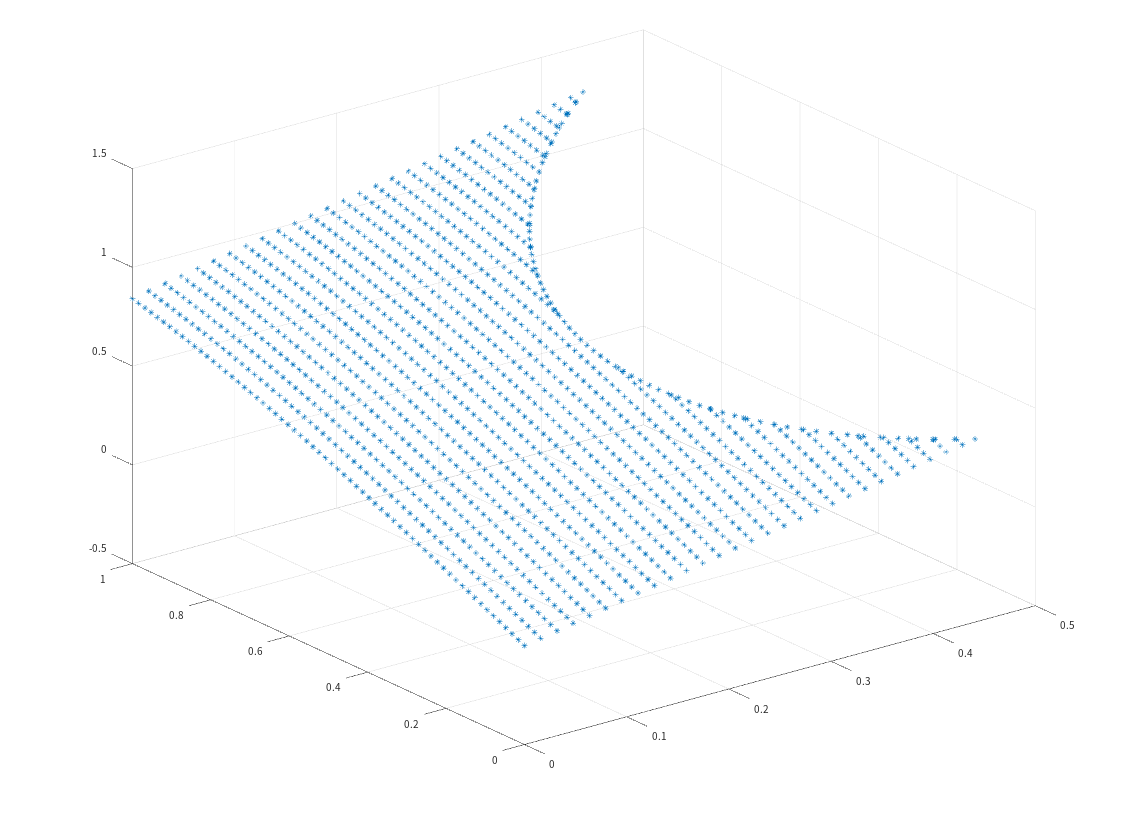
\includegraphics[width=0.8\textwidth,height=0.6\textwidth]{../output/image/image2.png}
\end{figure}

\subsection{The third function}
\par 测试的第三个函数是
$$ u(x,y) = x^2y $$
测试中不规则定义域中的圆选取为$(x-\frac{1}{2})^2+(y-\frac{1}{2})^2=(\frac{2}{7})^2$.
\par 对第一个边值条件,
\begin{center}
\begin{tabular}{|c|c|c|c|c|c|c|}
	\hline
	& \multicolumn{3}{c|}{regular domin} & \multicolumn{3}{c|}{irregular domin} \\
	\hline
	n & 1-norm & 2-norm & $\infty$-norm & 1-norm &	2-norm& $\infty$-norm \\
	\hline
	8& 1.03468e-15& 6.84845e-16 &9.99201e-16 & 3.4703e-15 & 3.10723e-15 & 5.88418e-15 \\
	\hline
	16& 1.69762e-15 & 1.05133e-15 & 2.44249e-15 & 1.17399e-13 &7.21967e-14&1.14742e-13\\
	\hline
	32& 6.07156e-15 & 2.25898e-15 & 4.88498e-15 & 9.30995e-13&8.65391e-13&3.20033e-12\\
	\hline
	64& 2.98187e-14 & 1.67381e-14 & 5.88418e-14 & 2.78576e-12 &1.38599e-12&4.63907e-12 \\
	\hline
\end{tabular}
\end{center}
\par 对第二个边值条件,
\begin{center}
\begin{tabular}{|c|c|c|c|c|c|c|}
	\hline
	& \multicolumn{3}{c|}{regular domin} & \multicolumn{3}{c|}{irregular domin} \\
	\hline
	n & 1-norm & 2-norm & $\infty$-norm & 1-norm &	2-norm& $\infty$-norm \\
	\hline
	8& 5.15866e-16& 2.37955e-16 &3.33067e-16 & 1.40043e-13 & 1.25456e-13 & 2.60291e-13 \\
	\hline
	16& 1.21707e-14 & 3.63509e-15 & 2.33147e-15 & 6.78763e-12 &6.74596e-12&2.22358e-11\\
	\hline
	32& 9.18311e-15 & 2.65691e-15 & 2.10942e-15 & 4.57356e-11&5.94086e-11&2.90419e-10\\
	\hline
	64& 7.32387e-14 & 1.13791e-14 & 3.55271e-15 &1.90752e-09&2.02197e-09&1.37753e-08 \\
	\hline
\end{tabular}
\end{center}
\par 对第三个边值条件,
\begin{center}
\begin{tabular}{|c|c|c|c|c|c|c|}
	\hline
	& \multicolumn{3}{c|}{regular domin} & \multicolumn{3}{c|}{irregular domin} \\
	\hline
	n & 1-norm & 2-norm & $\infty$-norm & 1-norm &	2-norm& $\infty$-norm \\
	\hline
	8& 2.51201e-15& 9.70023e-16 &3.33067e-16 & 0.191359 & 0.0744244 & 0.0482799 \\
	\hline
	16& 1.60553e-14 & 4.60769e-15 & 2.33147e-15 & 0.103656 &0.0307469&0.0149424\\
	\hline
	32&7.29843e-14& 1.49317e-14 & 5.44009e-15 & 0.122812&0.0286453&0.0130624\\
	\hline
	64& 3.35439e-14 & 6.74645e-15 & 4.21885e-15 &0.106139&0.0181115&0.00602779 \\
	\hline
\end{tabular}
\end{center}
\par 因为$u(x,y)=x^2y$关于$x$是2次的,关于$y$是1次的,因此前两个边值条件以及第三个边值条件的
规则定义域情况的计算都是准确的,只有机器误差。而第三个边值条件的不规则定义域情况的误差呈1阶收敛。
\par 绘制出在第二个边值条件及不规则定义域下,$n=64$时拟合出的函数图像如下:
\begin{figure}[H]
	\centering
	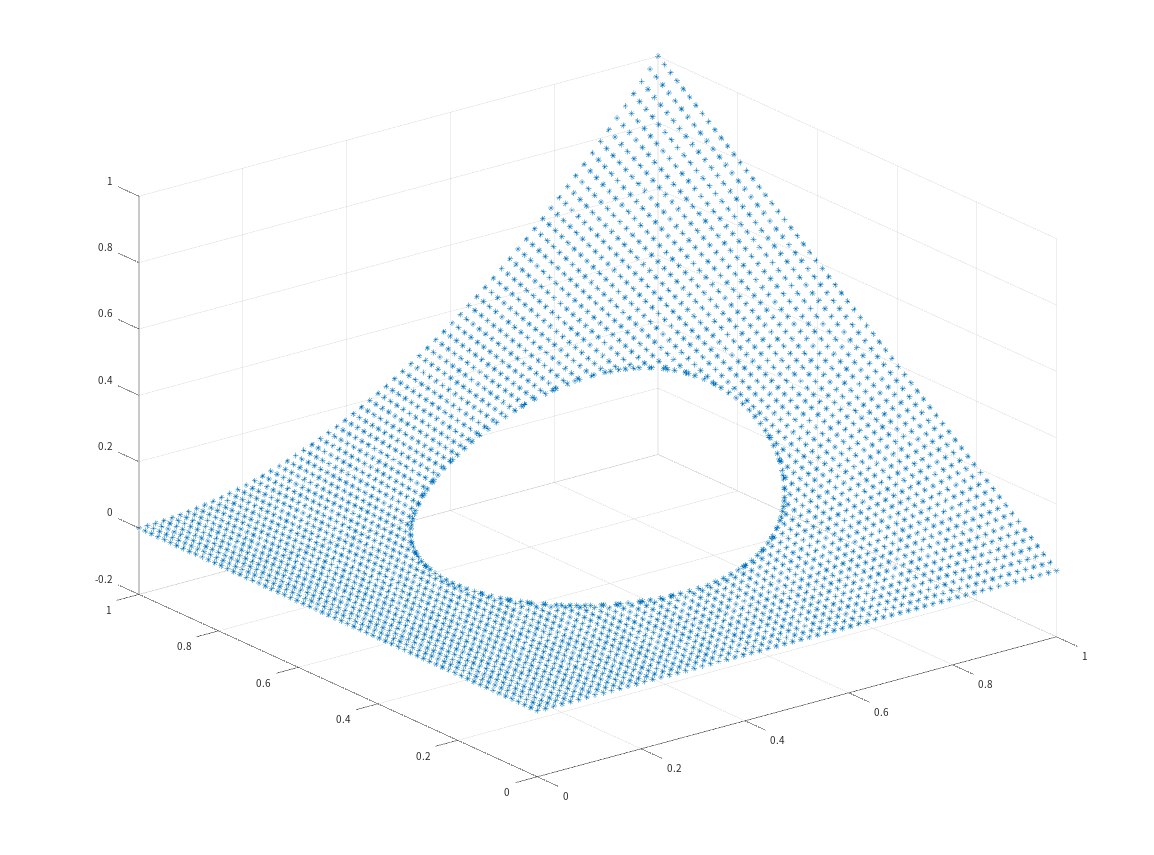
\includegraphics[width=0.8\textwidth,height=0.6\textwidth]{../output/image/image3.png}
\end{figure}



\end{large}
\end{document}